\begin{Aufgabe}[9]
	Die folgende Abbildung zeigt den Verlauf einer periodischen Funktion $f$:
	 
	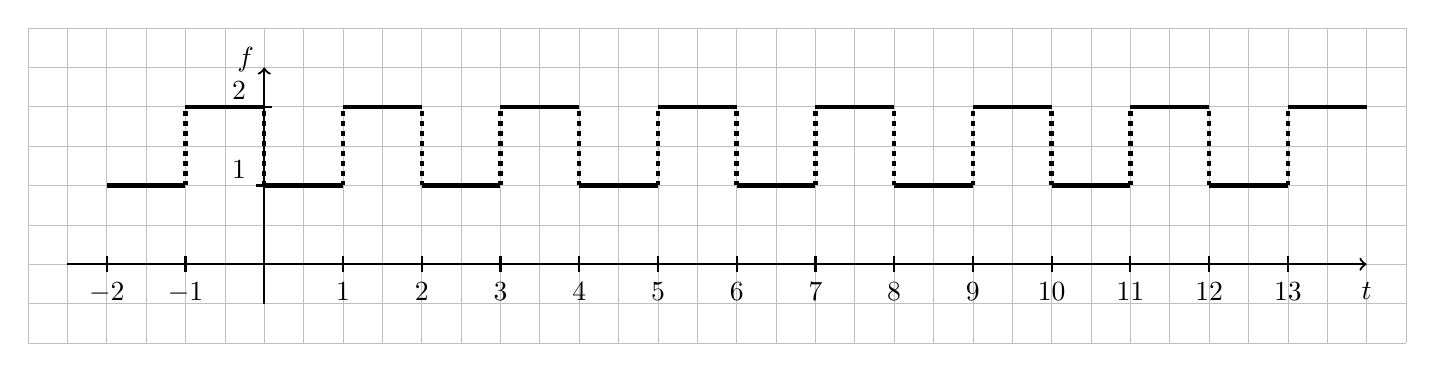
\begin{tikzpicture}[xscale=1.0,yscale=1.0]
		\draw[line width=0.25pt,step=0.5cm,color=lightgray] (-3.0,-1.0) grid(14.5cm,3.0cm);
		\draw[->,thick] (-2.5,  0.0) -- (14.0, 0.0) node[below=1mm] {$t$};
		\draw[->,thick] (  0.0,-0.5) -- ( 0.0,2.5) node[above=1mm,left]  {$f$};
		\foreach \i in {-2,-1,1,2,3,4,5,6,7,8,9,10,11,12,13} {
			\draw[thick] (\i,0.1) -- (\i,-0.1) node[below] {$\i$};
		}
		\foreach \i in {1,2} {
			\draw[thick] (0.1,\i) -- (-0.1,\i) node[above=2mm,left] {$\i$};
		}
		\foreach \i in {-1,0,1,2,3,4,5,6} {
			\draw[ultra thick] (2*\i,1) -- (2*\i+1,1);
			\draw[ultra thick] (2*\i+1,2) -- (2*\i+2,2);
		}
		\foreach \i in {-1,0,1,2,3,4,5,6,7,8,9,10,11,12,13} {
			\draw[ultra thick,dotted] (\i,1) -- (\i,2);
		}
	\end{tikzpicture}
	
	\begin{enumerate}
		\item
			Welche Periode $T$ und welche Kreisfrequenz $\omega$ hat die Funktion $f$?
		\item
			Ermitteln Sie den Mittelwert $m$ der Funktion $f$.
		\item
			Sind die Aussagen richtig oder falsch?
			Bitte kreuzen Sie den entsprechenden Eintrag an:
			
			\ifLoesung 
			\begin{tabular}{p{0.6\textwidth}p{0.1\textwidth}p{0.1\textwidth}}
				Alle reellen Fourier-Koeffizienten $a_k$ sind für $k>0$ null. & {\textcolor{red}X} richtig & $\square$             falsch\\
				Alle reellen Fourier-Koeffizienten $b_k$ sind für $k>0$ null. & $\square$             richtig & {\textcolor{red}X} falsch\\
			\end{tabular}
			\hfill\Punkte{1 P}
			\else
			\begin{tabular}{p{0.6\textwidth}p{0.1\textwidth}p{0.1\textwidth}}
				Alle reellen Fourier-Koeffizienten $a_k$ sind für $k>0$ null. & $\square$             richtig & $\square$             falsch\\
				Alle reellen Fourier-Koeffizienten $b_k$ sind für $k>0$ null. & $\square$             richtig & $\square$             falsch\\
			\end{tabular}
			\fi
		\item
			Berechnen Sie für $k>0$ eine Formel für die komplexen Fourier-Koeffizienten $c_k$.
		\item
			Geben Sie die Werte für die komplexen Fourier-Koeffizienten $c_1$ und $c_2$ explizit an.
	\end{enumerate}
	
	\Loesung{}{
		\begin{enumerate}[series=fourier]
			\item
				Periode $T=2$ und Kreisfrequenz $\omega = \pi$.
				\hfill\Punkte{1 P}
			\item
				Mittelwert:
				\hfill\Punkte{1 P}
				\[
					m = \frac{\mbox{Fläche einer Periode}}{\mbox{Periode}} = \frac{3}{2}
				\]
			\item
		\end{enumerate}
	}
		
	\newpage
		
	\Loesung{}{
		\begin{enumerate}[resume=fourier]
			\item
				Formel für $c_k$:
				\hfill\Punkte{1 P}
				\[
					c_k = \frac{1}{T}\int_{-T/2}^{T/2}f(t) \, \e^{-i \, k \, \omega \, t}\, \mathrm{d}t  = \frac{1}{2}\int_{-1}^1f(t) \e^{-i \, k \, \pi \, t}\, \mathrm{d}t 
				\]
				Aufspalten in zwei Teilintegrale:
				\hfill\Punkte{1 P}
				\[
					c_k = \frac{1}{2}\int_{-1}^0 1 \cdot \e^{-i \, k \, \pi \, t}\, \mathrm{d}t+\frac{1}{2}\int_{0}^1 2 \cdot \e^{-i \, k \, \pi \, t}\, \mathrm{d} t
				\]
				Stammfunktionen:
				\hfill\Punkte{1 P}
				\[
					c_k = \frac{1}{2}\Big[ \frac{\e^{-i \, k \, \pi \, t}}{-i \, k \, \pi} \Big]_{-1}^0 +\Big[ \frac{\e^{-i \, k \, \pi \, t}}{-i \, k \, \pi}\Big]_0^1
				\]
				Grenzen einsetzen:
				\hfill\Punkte{1 P}
				\[
					c_k = \frac{1}{2} \frac{1 - \e^{i \, k \, \pi}}{-i \, k \, \pi} + \frac{\e^{-i \, k \, \pi }-1}{-i \, k \, \pi}.
				\]
				Wegen $\e^{\pm i \, k \, \pi} = (-1)^k$:
				\hfill\Punkte{1 P}
				\[
					c_k = \frac{1-(-1)^k+2(-1)^k-2}{-2 \, i \, k \, \pi} = \frac{(-1)^k-1}{-2 \, i \, k \, \pi} = \frac{(-1)^k-1}{2 \, k \, \pi} \, i
				\]
			\item
				Für $k=1$ und $k=2$:
				\hfill\Punkte{1 P}
				\[
					c_1 = \frac{(-1)^1-1}{2 \cdot 1 \cdot \pi} \, i = -\frac{1}{\pi} \, i, \quad
					c_2 = \frac{(-1)^2-1}{2 \cdot 2 \cdot \pi} \, i = 0
				\]
		\end{enumerate}
	}
	
\end{Aufgabe}

\newpage

\endinput